\documentclass[12pt, twoside]{article}
\usepackage[letterpaper, margin=1in, head=30pt, headsep=0.1in]{geometry}
\usepackage[english]{babel}
\usepackage[utf8]{inputenc}
\usepackage{amsmath}
\usepackage{amsfonts}
\usepackage{amssymb}
\usepackage{tikz}
\usetikzlibrary{quotes, angles}

\usepackage{graphicx}
\usepackage{enumitem}
\usepackage{multicol}

%\usepackage{pgfplots}
%\pgfplotsset{width=10cm,compat=1.9}
%\usepgfplotslibrary{statistics}
%\usepackage{pgfplotstable}
%\usepackage{tkz-fct}
%\usepackage{venndiagram}

\usepackage{fancyhdr}
\pagestyle{fancy}
\fancyhf{}
\renewcommand{\headrulewidth}{0pt} % disable the underline of the header
\raggedbottom
\newif\ifmeta
\metatrue %print standards and topics tags

\title{Math AI Worksheet Generator and Formative Assessment System}
\author{Chris Huson}
\date{October 2020}

%\fancyhead[RE]{\thepage}
%\fancyhead[RO]{\thepage \\ Name: \hspace{3cm}}
%\fancyhead[L]{BECA / Dr. Huson / 10th Grade Geometry\\* 7 June 2019}
%
%\begin{document}
%\subsubsection*{13.7 Homework: Cross sections, distance applications}
%\fancyhead[L]{BECA / Dr. Huson / Geometry 03-Volume+angle-bisectors\\* pset ID: 34}

\begin{document}

\subsubsection*{3.1 Parallelogram and triangle area}
\begin{enumerate}

\item Do Now: The vertical line segment $\overline{PQ}$ is plotted on the coordinate plane with $P(4,8)$ and $Q(4,2)$. 
  \begin{multicols}{2}
    Find the length $PQ$. \\[0.5cm]
    Show the calculation, including the absolute value bars. Count on the grid as a check. (leave marks)
      \begin{flushright}
      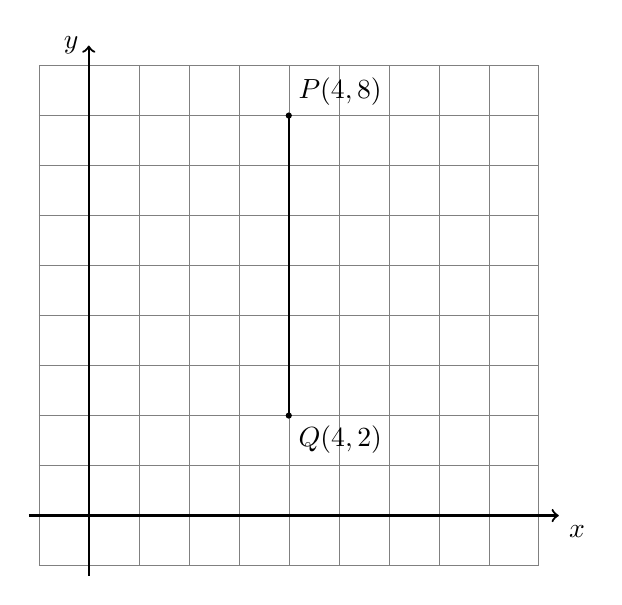
\begin{tikzpicture}[scale=.635]
        \draw [help lines] (-1,-1) grid (9,9);
        \draw [thick, ->] (-1.2,0) -- (9.4,0) node [below right] {$x$};
        \draw [thick, ->] (0,-1.2)--(0,9.4) node [left] {$y$};
        \draw [-, thick] (4,8)--(4,2);
        \draw [fill] (4,8) circle [radius=0.05] node[above right]{$P(4,8)$};
        \draw [fill] (4,2) circle [radius=0.05] node[below right]{$Q(4,2)$};
      \end{tikzpicture}
      \end{flushright}
  \end{multicols} 
  
\newpage
\item The horizontal line segment $\overline{RS}$ is plotted on the coordinate plane with $R(1,3)$ and $S(5,3)$. 
  \begin{multicols}{2}
    Find the length $RS$. \\[0.5cm]
    Show the calculation.
      \begin{flushright}
      \begin{tikzpicture}[scale=.635]
        %\draw [help lines] (-1,-1) grid (9,9);
        \draw [thick, ->] (-1.2,0) -- (9.4,0) node [below right] {$x$};
        \draw [thick, ->] (0,-1.2)--(0,6.4) node [left] {$y$};
        \draw [-, thick] (1,3)--(5,3);
        \draw [fill] (1,3) circle [radius=0.05] node[below]{$R(1,3)$};
        \draw [fill] (5,3) circle [radius=0.05] node[below right]{$S(5,3)$};
      \end{tikzpicture}
      \end{flushright}
  \end{multicols} 

\newpage
\item A parallelogram is shown on the $x$-$y$ plane having a base $b=4$ and height $h=3$. 
  \begin{multicols}{2}
    Find its area, showing the calculation.
      \begin{flushright}
      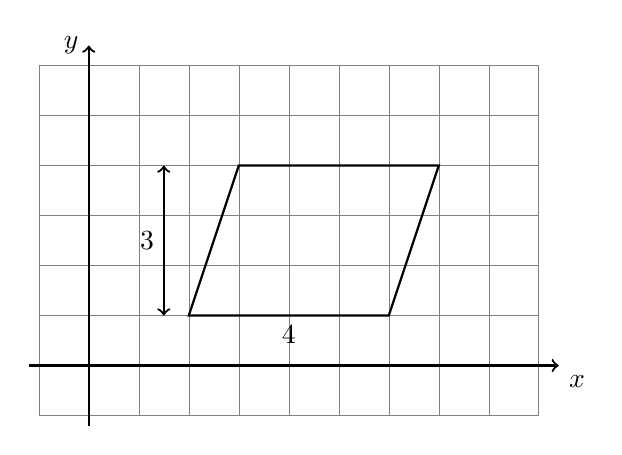
\begin{tikzpicture}[scale=.635]
        \draw [help lines] (-1,-1) grid (9,6);
        \draw [thick, ->] (-1.2,0) -- (9.4,0) node [below right] {$x$};
        \draw [thick, ->] (0,-1.2)--(0,6.4) node [left] {$y$};
        \draw [<->, thick] (1.5,1)--(1.5,4);
        \draw [-, thick] (2,1)--(6,1)--(7,4)--(3,4)--cycle;
        \node at (4,1)[below]{$4$};
        \node at (1.5,2.5)[left]{$3$};
      \end{tikzpicture}
      \end{flushright}
  \end{multicols} 

\newpage
\item The $\triangle ABC$ is shown below with $A(2,1)$, $B(7,1)$, and $C(1,5)$. The length of the base of the triangle is $AB=5$.
  \begin{multicols}{2}
    \begin{enumerate}
      \item Find the height $h$.
      \item Find its area, showing the calculation. \vspace{2cm}
      \end{enumerate}
      \begin{flushright}
      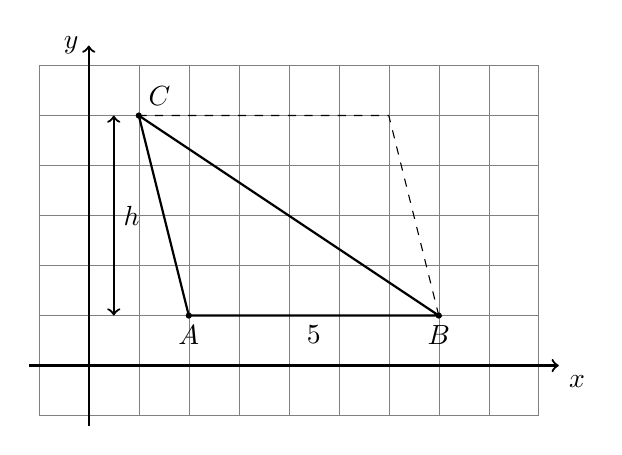
\begin{tikzpicture}[scale=.635]
        \draw [help lines] (-1,-1) grid (9,6);
        \draw [thick, ->] (-1.2,0) -- (9.4,0) node [below right] {$x$};
        \draw [thick, ->] (0,-1.2)--(0,6.4) node [left] {$y$};
        \draw [<->, thick] (0.5,1)--(0.5,5);
        \draw [-, thick] (2,1)--(7,1)--(1,5)--cycle;
        \draw [-, dashed] (7,1)--(6,5)--(1,5);
        \draw [fill] (2,1) circle [radius=0.05] node[below] {$A$};
        \draw [fill] (7,1) circle [radius=0.05] node[below] {$B$};
        \draw [fill] (1,5) circle [radius=0.05] node[above right] {$C$};
        \node at (4.5,1)[below]{$5$};
        \node at (0.5,3)[right]{$h$};
      \end{tikzpicture}
      \end{flushright}
  \end{multicols} 

\newpage
\item Spicy: Find the area of the $\triangle ABC$ is shown below with $A(3,2)$, $B(7,4)$, and $C(4,8)$. 
  \begin{multicols}{2}
    \begin{enumerate}
      \item First find the area of the red rectangle with sides $b=4$, $h=6$.
      \item Find the area of the three triangles surrounding $\triangle ABC$ in the rectangle. 
      \item Subtract their areas from the rectangle to find $A_{\triangle ABC}$
      \end{enumerate}
      \begin{flushright}
      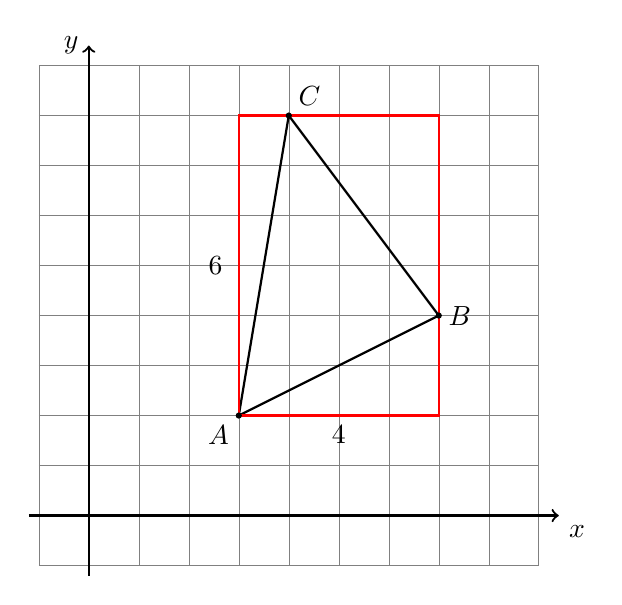
\begin{tikzpicture}[scale=.635]
        \draw [help lines] (-1,-1) grid (9,9);
        \draw [thick, ->] (-1.2,0) -- (9.4,0) node [below right] {$x$};
        \draw [thick, ->] (0,-1.2)--(0,9.4) node [left] {$y$};
        %\draw [<->, thick] (0.5,1)--(0.5,5);
        \draw [-, thick] (3,2)--(7,4)--(4,8)--cycle;
        \draw [-, thick, red] (3,2)--(7,2)--(7,8)--(3,8)--cycle;
        \draw [fill] (3,2) circle [radius=0.05] node[below left] {$A$};
        \draw [fill] (7,4) circle [radius=0.05] node[right] {$B$};
        \draw [fill] (4,8) circle [radius=0.05] node[above right] {$C$};
        \node at (5,2)[below]{$4$};
        \node at (2.2,5)[right]{$6$};
      \end{tikzpicture}
      \end{flushright}
  \end{multicols} 

\end{enumerate}
\end{document}